\section{Frequency-domain subspace identification}
\label{sec:freq-doma-subsp}

This section describes a methods for estimation of the underlying linear
frequency response function and nonlinear coefficients for nonlinear systems.
The method is an (nonlinear) extension of linear subspace methods which are able
to deal with multiple-input, multiple-output(MIMO) systems.

The nonlinear subspace methods interpret nonlinearities as unmeasured internal
forces, ie. nonlinearities are seen as cause of distortion on the linear FRF
matrix. Two main nonlinear methods exist, one in time domain: time-domain
subspace identification (TNSI)\autocite{marchesiello2008a} and one in frequency
domain: frequency-domain subspace identification (FNSI)\autocite{noel2013a} .
Both performs equally well in identification and robustness, but the main
benefit of FNSI is that the input time series, when converted to frequency
domain, can be truncated to a frequency interval of interest and thus reduce the
computational time. FNSI is the method used here.



Given the equation of motion for a dynamical system with nonlinearities:

\begin{equation}
  \label{eq:EOM_fnsi}
  \bm M \ddot{\bm q}(t) + \bm C \dot{\bm q}(t) + \bm K \bm q(t) +
  \bm f_{nl} \left( \bm q(t), \dot{ \bm q}(t) \right) = \bm p (t)
\end{equation}

where $\bm M$, $\bm C$ and $\bm K \in \mathbb{R}^{n \times \, n}$ are the
mass, linear viscous damping and linear stiffness matrices; $\bm q(t)$ and
$\bm p(t) \in \mathbb{R}^{n}$ are the generalised displacement and external
force vectors; $\bm f_{nl}(t) \in \mathbb{R}^{n}$ is the essentially nonlinear,
i.e. nonlinearisable, restoring force vector comprising elastic and dissipative
contributions; $n$ is the number of DOFs.


The notation of \eqref{eq:EOM_fnsi} assumes that all linear components of the
restoring forces in the system are included in the matrices $\bm K$ and $\bm
C$. The nonlinear restoring force is expressed by a linear combination of $s$
lumped nonlinearities

\begin{equation}
  \label{eq:nonlin_fnsi_lummped}
  \bm f_{nl} \left( \bm q(t), \dot{\bm q}(t) \right) =
  \sum_{i=1}^s \mu_i \bm b_i \bm g_i \left( \bm q(t), \dot{\bm q}(t) \right)
\end{equation}
where $\mu_i$ is the unknown nonlinear coefficient and $\bm g_i \left( \bm q(t),
  \dot{\bm q}(t) \right)$ is the the corresponding known (identified by eg. RFS)
functional form (or basis function). The location of the nonlinearity is
specified by the boolean vector, $\bm b_i \in \mathbb{R}^{n}$.


Moving the nonlinear terms of \eqref{eq:EOM_fnsi} to the right-hand side

\begin{equation}
  \label{eq:EOM_fnsi_final}
  \bm M \ddot{\bm q}(t) + \bm C_v \dot{\bm q}(t) + \bm K \bm q(t) = -
  \sum_{i=1}^s \mu_i \bm b_i \bm g_i(t) + \bm p(t)
\end{equation}
the system may be viewed as the underlying linear system subjected to the
external force $\bm p(t)$ and the internal feedback force due to nonlinearities,
as shown in figure \ref{fig:fnsi_feedback}.

\begin{figure}[!ht]
  \centering
  % \import{fig/fnsi/}{fnsi_feedback.pdf_tex}
  % 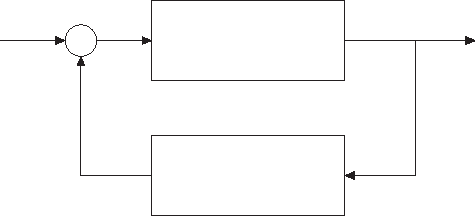
\includegraphics[width=0.5\textwidth]{fnsi/fnsi_feedback}
  \tikzstyle{block} = [draw, fill=white, rectangle, minimum height=3em, minimum width=6em]
  \tikzstyle{sum} = [draw, fill=white, circle, node distance=1.5cm, plus]
  \tikzstyle{input} = [coordinate]
  \tikzstyle{output} = [coordinate]
  \begin{tikzpicture}[auto, node distance=2cm,>=latex']
    \node [input, name=input] {};
    \node [sum, right of=input] (sum) {};
    \node [block, right=1cm of sum, align=left] (system)
      {Underlying linear\\ system: $\bm M, \bm C, \bm K$};
    \node [output, right=2cm of system] (output) {};
    \node [block, below of=system, align=left] (feedback)
      {Nonlinear feedback:\\ $c_a, \bm g_a(\bm y_{nl}(t), \dot{\bm y}_{nl}(t))$};
    \draw [draw,->] (input) -- node {$\bm u(t)$} (sum);
    \draw [->] (sum) -- node {} (system);
    \draw [->] (system) -- node [name=y] {$\bm y, \dot{\bm y}$}(output);
    \draw [-] (y) |- (feedback);
    \draw [->] (feedback) -| node [near end] {} (sum);
  \end{tikzpicture}
  \caption{Feedback interpretation of nonlinear structural dynamics.}
  \label{fig:fnsi_feedback}
\end{figure}


Using the state vector $\bm x = [\bm q, \dot{\bm q}]^T\in\mathbb{R}^r$, the
system \eqref{eq:EOM_fnsi_final} is rewritten as the state space formulation
\begin{equation}
  \label{eq:fnsi_c_state_space}
  \begin{split}
    &\dot{\bm x}(t) = \bm A_c \bm x(t) + \bm B_c \bm e(t) \\
    &\bm y(t) = \bm C \bm x(t) + \bm D \bm e(t)
  \end{split}
\end{equation}
where subscript $c$ denotes {\textit continuous time} and $r=2n$. $\bm e(t) =
\bm p(t)^T, g_1, \dots , g_s]^T \in \mathbb{R}^{n+s}$ is the extended input
vector which concatenates external and nonlinear terms.

State-space and physical matrices have the relations
\begin{equation}
  \label{eq:state_to_physical_mat}
  \begin{split}
  \bm A_c =
  \begin{bmatrix}
    \bm O^{r \times r} & \bm I^{r \times r} \\
    -\bm M^{-1}K     & -\bm M^{-1} \bm C \\
  \end{bmatrix}
  \in \mathbb{R}^{2r \times 2r} , \\
  \bm B_c =
  \begin{bmatrix}
    \bm 0^{r \times 1} & \bm 0^{r \times 1} & ... &
    \bm 0^{r \times 1} & \bm 0^{r \times 1} \\
    -\mu_1 \bm M^{-1} \bm b_1 & -\mu_2 \bm M^{-1} \bm b_2 & ... &
    -\mu_s \bm M^{-1} \bm b_S & -\mu_1 \bm M^{-1} \bm b_1 & \\
  \end{bmatrix}
  \in \mathbb{R}^{(n \times \sigma)} \\
  \bm C =
  \begin{bmatrix}
    \bm I^{n\times n} & \bm I^{n\times n}
  \end{bmatrix}
  \in \mathbb{R}^{(n \times n)} \,\quad
  \bm D = \bm 0^{n\times\sigma}
\end{split}
\end{equation}
The state matrices are: $\bm A$ and $\bm B$ the input and nonlinear coefficients
matrix, the output matrix $\bm C$ and the direct feed through matrix $\bm D$.

This way of characterizing the system above is the same as with TNSI. Using a
Fourier transform, the system is

\begin{equation}
  \label{eq:fnsi_freq_state}
  \begin{aligned}
    z_k \bm X &= \bm A_d \bm X(k) + \bm B_d \bm E(k) \\
    \bm Y(k) &= \bm C \bm X(k) + \bm D \bm E(k)
\end{aligned}
\end{equation}
where $z_k = e^{(2i\pi k/N_s)}$ is the Z-transform variable for discrete time
models and $N_s$ the number of recorded samples in the time series. $\bm X, \bm
Y$ and $\bm E$ are the discrete Fourier transforms of $\bm x, \bm y$ and $\bm e$.

\textbf{Noget om at fitte en discrete time model til continuous time for sikre
  good conditioning}

\subsection{The output-state-input equation}

The extended input $\bm E$ and output $\bm Y$ is known. The system matrices $\bm
A_d, \bm B_d, \bm C$ and $\bm D$ needs to be determined along with the system
order $r$. Frequency-domain subspace methods estimates these matrices based on a
reformulation of the state-space eqs. \eqref{eq:fnsi_freq_state} in matrix form.
The matrix of the measured output spectra is

\begin{equation}
  \bm Y_i =
  \begin{bmatrix}
    \bm Y(1) & \bm Y(2) & \dots & \bm Y(N) \\
    z_1\bm Y(1) & z_2\bm Y(2) & \dots & z_F\bm Y(N) \\
    z^2_1\bm Y(1) & z^2_2\bm Y(2) & \dots & z^2_F\bm Y(N) \\
    \vdots \\
    z^{i-1}_1\bm Y(1) & z^{i-1}_2\bm Y(2) & \dots & z^{i-1}_F\bm Y(N)
  \end{bmatrix}
\end{equation}
which by defining $\xi = \text{diag}(z_1, z_2, \dots, z_N)$ is recast to

\begin{equation}
  \begin{aligned}
    \bm Y_i =
    \begin{bmatrix}
      \bm Y^T & (\bm Y \xi)^T & \dots & (\bm Y \xi^{i-1})^T
    \end{bmatrix}^T \\
    \bm E_i =
    \begin{bmatrix}
      \bm E^T & (\bm E \xi)^T & \dots & (\bm E \xi^{i-1})^T
    \end{bmatrix}^T
  \end{aligned}
\end{equation}
where $i$ is the user-defined number of block rows in $\bm Y_i$ and $N$ the
number of frequency lines used for identification.

Introducing the extended observability matrix
\begin{equation}
  \bm \Gamma_i =
  \begin{bmatrix}
    \bm C^T & (\bm C \bm A)^T & \dots & (\bm C \bm A^{i-1})^T
  \end{bmatrix}^T
\end{equation}
and the lower-block triangular Toeplitz matrix

\begin{equation}
  \bm H_i =
  \begin{bmatrix}
    \bm D                   & \bm 0                   & \bm 0                   & \dots & \bm 0 \\
    \bm C \bm B             & \bm D                   & \bm 0                   & \dots & \bm 0 \\
    \bm C \bm A \bm B       & \bm C \bm B             & \bm D                   & \dots & \bm 0 \\
    \vdots \\
    \bm C \bm A^{i-2} \bm B & \bm C \bm A^{i-3} \bm B & \bm C \bm A^{i-3} \bm B & \dots & \bm D
  \end{bmatrix}^T
\end{equation}

By recursive use of eq. \eqref{eq:fnsi_freq_state} \autocite{noel2013a}, the
output-state-input matrix equation, which is used for estimation in the subspace
method, is obtained
\begin{equation}
  \label{eq:fnsi_state_matrix}
  \bm Y_i = \bm \Gamma_i \bm X + \bm H_i \bm E_i
\end{equation}


\subsection{Estimation of state matrices}

The subspace method is applied to eq. \eqref{eq:fnsi_state_matrix} in order to
estimate $\bm \Gamma_i$ and the system order $n_s$. When $\bm \Gamma_i$ is
estimated, the state matrices of eq. \eqref{eq:fnsi_freq_state} are extracted
and calculated.

The method have two main steps:
\begin{itemize}
\item Eliminate the term depending on nonlinearities and forces in eq.
  \eqref{eq:fnsi_state_matrix}. This is done by projecting the equation onto the
  orthogonal complement of $\bm E_i$,
  \begin{equation}
    \bm Y_i / \bm E_i^\perp = \bm \Gamma_i \bm X / \bm E_i^\perp = \mathcal{P}
  \end{equation}
  The geometrical interpretation of this is shown in figure
  \ref{fig:fnsi_geometric} for the 2d case.

  $\Gamma_i$ is then estimated from a singular value decomposition(SVD) of the
  projection $\mathcal{P}$
\item When $\Gamma_i$ is estimated, the four state space matrices ($\bm A, \bm
  B, \bm C, \bm D$) are calculated. See figure \ref{fig:fnsi_methodolgoy} for a
  overview and \autocite{noel2013a} for more details.
\end{itemize}

\begin{figure}[!ht]
  \centering
    %\def\svgwidth{3cm}
  \import{fig/fnsi/}{fnsi_geometric2.pdf_tex}
  \caption{Geometric interpretation of eq. \eqref{eq:fnsi_state_matrix} in two
    dimensional space. The orthogonal complement of $\bm E_i$, $\bm E_i^\perp$,
    is the set of all vectors that are orthogonal to every vector of $\bm E_i$
    (thus it is also the null space of $\bm E_i$).
    In the 2d case, $\bm E_i^\perp$ is simply the vector perpendicular to $\bm
    E_i$, and the projection of $\bm Y_i$ cancels the extended input term $\bm
    H_i \bm E_i$. In 3d the orthogonal complement of the plane spanned of two
    vectors $\bm u$ and $\bm v$, is the subspace formed by all normal vectors to
    that plane.
  }
  \label{fig:fnsi_geometric}
\end{figure}


\begin{figure}[!ht]
  \centering
  \begin{mdframed}
    \begin{enumerate}
    \item Choose the index $i$ and the number of processed frequency lines N
    \item Concatenate external forces and nonlinearities to form the extended
      input spectra $E_i$
    \item Compute the orthogonal projection
      \begin{equation*}
        \mathcal{P} = \bm Y_i / \bm E_i^\perp
      \end{equation*}
      using QR-decomposition.
    \item Compute the SVD of $\mathcal{P}$
      \begin{equation}
        \label{eq:fnsi_svd}
        \mathcal{P} = \bm U \bm S \bm V
      \end{equation}
    \item Determine model order $n_s$ from singular values in $\bm S$ or from a
      stabilisation diagram. Truncate $\bm U$ and $\bm S$ accordingly to define
      $\bm U_1$ and $\bm S_1$.
    \item Estimate the extended observability matrix $\bm \Gamma_i$
      \begin{equation*}
        \hat{\bm \Gamma}_i = \bm U_1 \bm S_1^{1/2}
      \end{equation*}
    \item Estimate $\bm A$ using the shift property of $\bm \Gamma_i$,
      \begin{equation*}
        \underline{\bm \Gamma_i} \hat {\bm A} = \overline{\bm \Gamma_i}
        \iff
        \hat {\bm A} = \underline{\bm \Gamma^+_i} \overline{\bm \Gamma_i}
      \end{equation*}
      where $\underline{\bm \Gamma_i}$ and $\overline{\bm \Gamma_i}$ are the
      matrix $\bm \Gamma_i$ without its first and last $l$ rows.
      $\bm C$ is extracted as the first block row of $\bm \Gamma_i$.
    \item Estimate $\bm B$ and $\bm D$ by defining the transfer function matrix
      $\bm G_s$,
      \begin{equation*}
        \bm G_s(k) = \bm C(z_k \bm I - \bm A)^{-1} \bm B + \bm D
      \end{equation*}
      and minimise the difference between the measured and modelled output
      spectra in a linear least square sense, i.e.
      \begin{equation*}
        \hat {\bm B}, \hat {\bm D} = \arg \min_{\bm B, \bm D} \sum_{k=1}^F |\bm Y(k) - \bm G_s(k) \bm E(k)|^2
      \end{equation*}
    \item Convert $\bm A, \bm B, \bm C$ and $\bm D$ into continuous-time
      matrices and form the extended FRF $\bm H^e(\omega)$.
      \begin{equation}
        \label{eq:extend_FRF_He}
        \bm H^e(\omega) = \bm C_c \left(j \omega \bm I^{n \times n} - \bm A_c \right)^{-1} \bm B_c^e + \bm D_c^e
        \in \mathbb{C}^{(l \times \sigma)}
      \end{equation}
    \item Estimate the nonlinear coefficients $\mu_j$ and the linear FRF matrix
      $\bm H(\omega)$.
      The FRF matrix of the underlying linear system $\bm H(\omega) \in \mathbb{C}^{(l
        \times l)}$ and the nonlinear coefficients $\mu_s$ are found from
      \eqref{eq:extend_FRF_He} as
      \begin{equation}
        \label{eq:FRE_H}
        \bm Q(\omega) = \bm H(\omega)
        \begin{Bmatrix}
          \bm I^{l\times 1} & -\mu_1\bm b_1 & ... & -\mu_s \bm b_s
        \end{Bmatrix}
        \bm E (\omega)
        =
        \bm H^e(\omega) \bm E(\omega)
      \end{equation}
    \end{enumerate}
  \end{mdframed}
  \caption{Overview of the FNSI methodology}
  \label{fig:fnsi_methodolgoy}
\end{figure}



Three assumptions are assumed to be fulfilled for the subspace methods,
\begin{enumerate}
\item All the linear modes of vibration in the frequency band of interest are
  excited or, alternatively, they are all observable in input-output data.
\item The row space of the states $\bm X$ and of the extended input spectra
  matrix $\bm Y_i$ does not share information,
  \begin{equation*}
    \text{span}_{\text{row}} (\bm X) \cap \text{span}_{\text{row}}(\bm E_i) = 0
  \end{equation*}
\item The extended inputs $\bm E_i$ are of full rank, i.e.,
  \begin{equation*}
    \text{rank}(\bm E_i) = \sigma i
  \end{equation*}
  Excitations and the nonlinearities have to be such that the inversion of the
  problem is well-posed
\end{enumerate}

To expand on the second assumption:
The state term $\bm A \bm X$ contains linear stiffness and damping information.
If constant and/or linear terms are introduced in the nonlinear basis functions,
the intersection between the states and the extended inputs $\bm E_i$ is no
longer empty, which violate the assumption.
This requires nonlinear basis functions to be nonlinearisable, i.e. they should
be zero and have zero slope at the origin.



{\textbf Dimension:}

$\bm b_s \in \mathbb{R}^l$ is a boolean vector specifying the location of the
nonlinearity $\mu_s$.
$\sigma = m + s$, where $s$ is the number of lumped nonlinearities and $m \leq
r$ is the number of {\textit measured applied forces}. $l \leq r$ is the number of
{\textit measured applied displacement}.
$n$ is the model order, not $n=2r$ as used in the beginning of the article, and
$r$ is number of DOFs.



\subsection{Types of nonlinear functional}
\label{sec:fnsi_functional}


As stated, the nonlinear basis functions should be zero and have zero slope at
the origin. For continuous nonlinear restoring force, polynomial functions with
order chosen from RFS-plots can be used. For discontinuous systems, e.g. contact
polynomials might not be well suited, for instance higher order polynomials
exhibit oscillations around the origin. An alternative is to use piecewise cubic
spines instead. Even if they cannot realise a perfect fitting (they are
continuous by nature), they are appropriate for representing sudden events,
like sharp changes in stiffness/damping curves.

In order to get the basis functions from cubic splines, the abscissas of knots
is specified on beforehand and the ordinate as free parameters. FNSI then
estimate the ordinate.
Choosing the number of knots and their abscissas should rigorously be sought by
minimising the difference in some metric between the predictions of the
non-linear model and measured data. In reality it is still done by trial and
error.

Using cubic splines might be termed \textit{gray box} identification where using
polynomials is \textit{white box}. The difference is that with gray box, the
nonlinearities are described by functionals that may represent a vast variaty of
nonlinear behaviour and thus requiring less specific knowledge of the underlying
physics.


\subsection{Estimating model order}

In the presence of non-linearities, the model order translates the number of
underlying linear modes excited in the output data. This implies that, similarly
to linear system identification, a stabilisation analysis can be utilised as
decision-making tool instead of looking at the singular values of $\bm S$,
\eqref{eq:fnsi_svd}. The stabilisation diagram shows the stabilisation of the
estimated linear parameters: stabilisation in frequency, stabilisation in
damping and stabilisation of the mode. If all three parameters are stabilised
the mode is full stabilised. Stabilisation is compared to the same mode for one
model order higher. Stabilisation for the mode is calculated by the modal
assurance criterion(MAC) \autocite{Allemang2003},

\begin{equation}
  MACX(r,q) = \frac{|\bm \psi^T_r \bm \psi^*_q|^2}
  {\left( \bm \psi^T_r \bm \psi^*_r \right)\left( \bm \psi^T_q \bm \psi^*_q \right)}
\end{equation}

% For simulated data without noise, tolerances for frequency, damping and mode
% stabilisation are $0.5\%, 2\%, 0.98$ respectively.


If the model order is chosen too low, it will result in unmodelled dynamics,
whereas too large orders lead to overmodelling issues such as an increase of the
noise sensitivity of the model. It should be noted that model selection requires
that adequate basic functions are used.

Without anticipating the example, a stabilisation diagram for the coupled
duffing system is shown in figure \ref{fig:fnsi_stab} along with singular values
of $\bm S$ in figure \ref{fig:fnsi_svg}. The two modes are clearly seen.
From the stabilisation diagram a model order of four is chosen. This gives
stabilisation in the linear parameters. The plot of the singular values shows a
jump of six orders magnitude between model order four and five, verifying the
chosen model order.
In general only the stabilisation diagram is used; the singular value plot is
only used if a stabilisation diagram is not implemented.

\begin{figure}
  \centering
  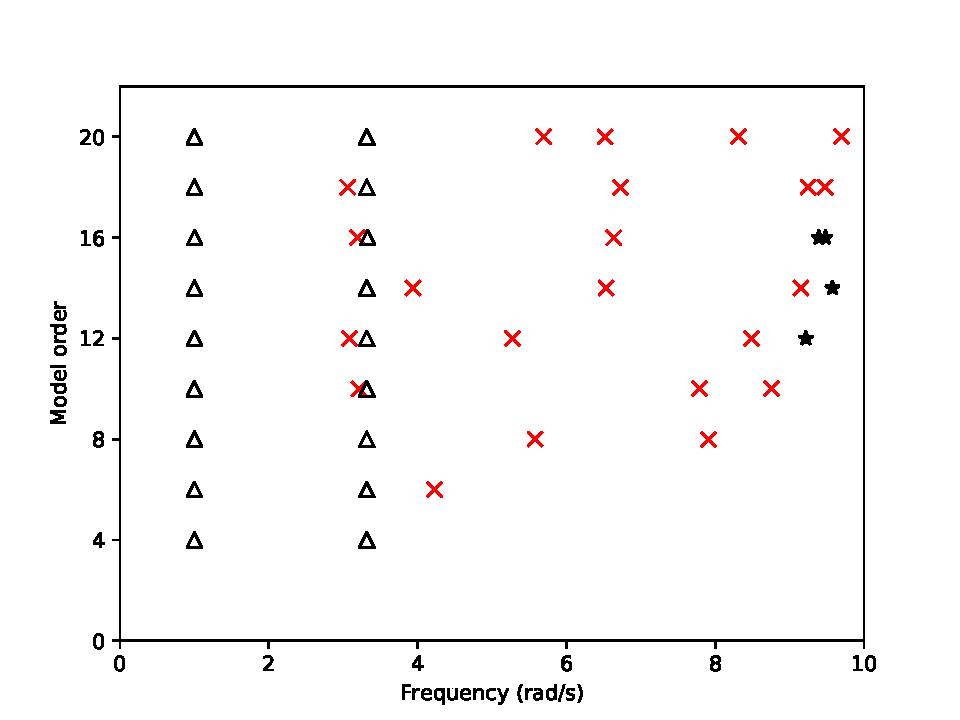
\includegraphics[width=0.8\linewidth]{fnsi/vrms3_stab.tikz}
  \caption{Estimation of model order. Stabilisation diagram with linear FRF overlayed.
    $\pmb\times$(red): new pole;
    $\pmb\star$: stabilisation in natural frequency;
    $\pmb\square$: extra stabilisation in damping ratio;
    $\pmb\circ$: extra stabilisation in MACX;
    $\pmb\triangle$: full stabilisation.
    Stabilisation thresholds in natural frequency, damping ratio and MACX value
    are $0.5\%, 2\%, 0.98$, respectively. Not all types of stabilisation are
    present here.
  }
  \label{fig:fnsi_stab}
\end{figure}

\begin{figure}
  \centering
  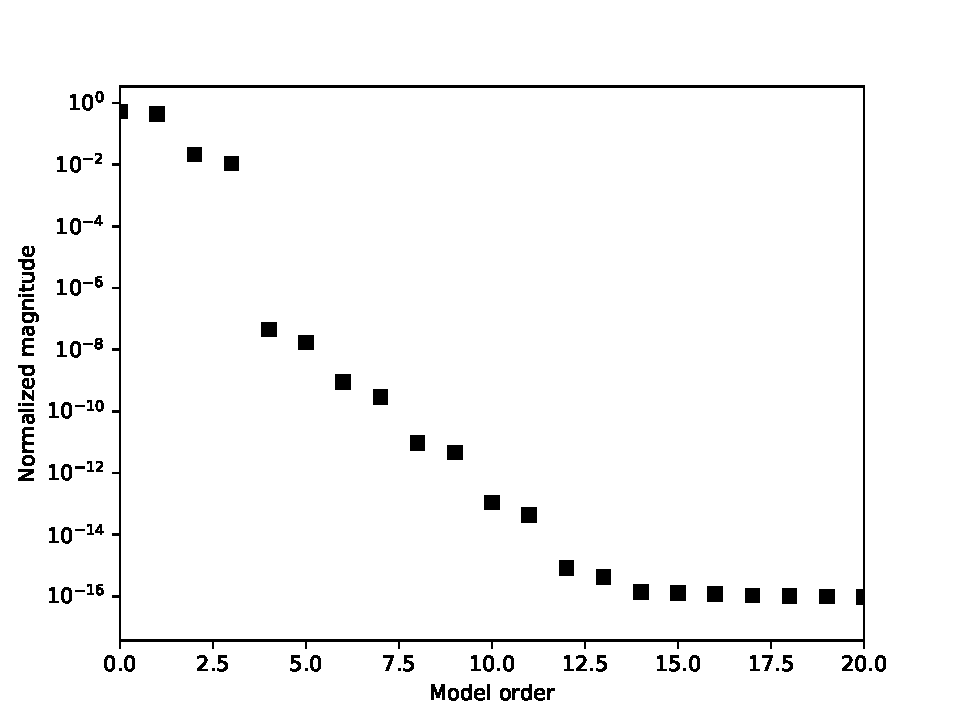
\includegraphics[width=0.6\linewidth, height=6cm]{fnsi/vrms3_svg.tikz}
  \caption{First tventy singular values. A jump of six orders magnitude is seen
    between model order four and five.}
  \label{fig:fnsi_svg}
\end{figure}

The determination of the model order is very simple and clear here. For larger system this
might not be the case, as seen with the more involved examples in section
\ref{cha:application}.

\subsection{Example}
\label{sec:fnsi_example}


Figure \ref{fig:periodicity} shows the periodicity of the recorded signal. The
signal of the last recorded period is compared to previous periods. For
identification, multiple periods can be used but transient effects should not be
present; which is indicated by a low periodicity.

\begin{figure}[!ht]
  \centering
  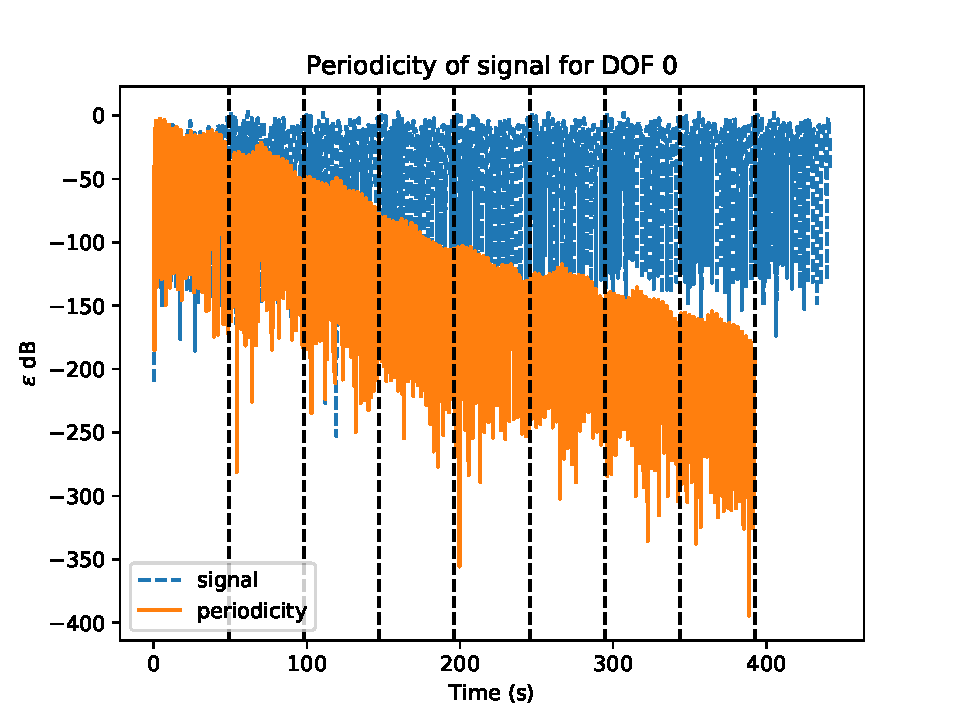
\includegraphics[width=0.7\linewidth]{signal/frf_per}
  \caption{Periodicity of recorded signal at DOF 0. Vertical lines indicate
    periods. A low periodicity shows that transient effects have died out}
  \label{fig:periodicity}
\end{figure}


The estimation of the nonlinear parameters of the coupled duffing system is
shown in figure \ref{fig:fnsi_knl} for model order four. The variation of the
real part of$\mu$ is shown in a 1\% interval, with very little frequency
dependency in the frequency range of interest. The imaginary part is about three
orders of magnitude smaller. Both indicates a good quality of the estimation.
The spectral averages are
\begin{equation}
  \begin{aligned}
    \Re (\mu_1) = 1.000, \quad \Im (\mu_1) = 1.09 \times 10^{-4} \\
    \Re (\mu_2) = 1.000, \quad \Im (\mu_1) = 7.73 \times 10^{-4}
  \end{aligned}
\end{equation}
matching the simulated values well.

\begin{figure}[!ht]
  \centering
  \begin{subfigure}[b]{0.45\textwidth}
    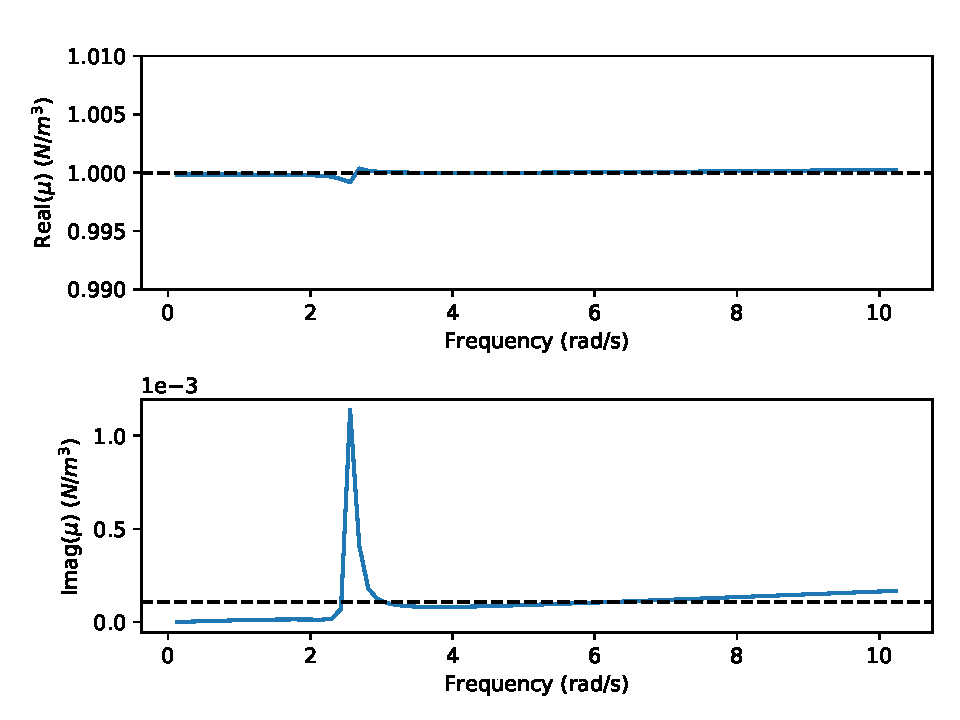
\includegraphics[width=\linewidth]{fnsi/vrms3_knl0.tikz}
    \caption{}
  \end{subfigure}
  ~
  \begin{subfigure}[b]{0.45\textwidth}
    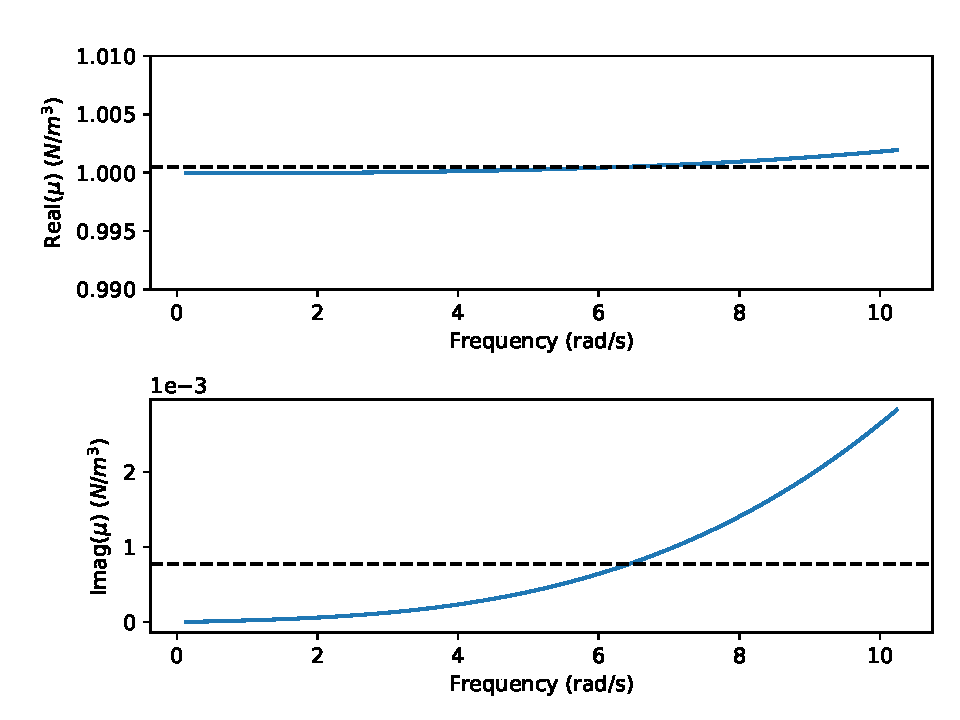
\includegraphics[width=\linewidth]{fnsi/vrms3_knl1.tikz}
    \caption{}
  \end{subfigure}
  \caption{Real and imaginary part of estimated nonlinear coefficients $\mu_1$
    and $\mu_2$. The variation of Re($\mu$) is shown in a 1\% interval, with
    very little frequency dependency in the frequency range of interest.
    The imaginary part is about three orders of magnitude smaller. Both
    indicates a good quality of the estimation.
    \textbf{(a)}: $\mu_1$;
    \textbf{(b)}: $\mu_2$.
  }
  \label{fig:fnsi_knl}
\end{figure}

The FNSI method also estimate the underlaying linear properties. As seen from
table \ref{tab:fnsi_eigen}, the linear parameters are identified correctly.
Ensuring that linear parameters are identified, also shows that nonlinear
coefficients are identified correct.

\begin{center}
  \begin{tabular}{*{3}{c}}
    \hline
    Mode & Frequency (rad/s) & Damping ration (\%) \\
    1 & 1.00 & 5.00 \\
    2 & 3.32 & 1.51 \\
    \hline
    1 & 1.19 & 3.96 \\
    2 & 3.40 & 1.41 \\
    \hline
  \end{tabular}
  \captionof{table}{Estimated linear natural frequencies and damping ratios for
    the coupled Duffing system.
    \textbf{(upper)}: Nonlinear identification with FNSI;
    \textbf{(lower)}: Linear identification
  }
  \label{tab:fnsi_eigen}
\end{center}

Figure \ref{fig:fnsi_H1} shows the transfer function. The linear transfer
function found by FNSI match the theoretical linear transfer function.

\begin{figure}[!ht]
  \centering
  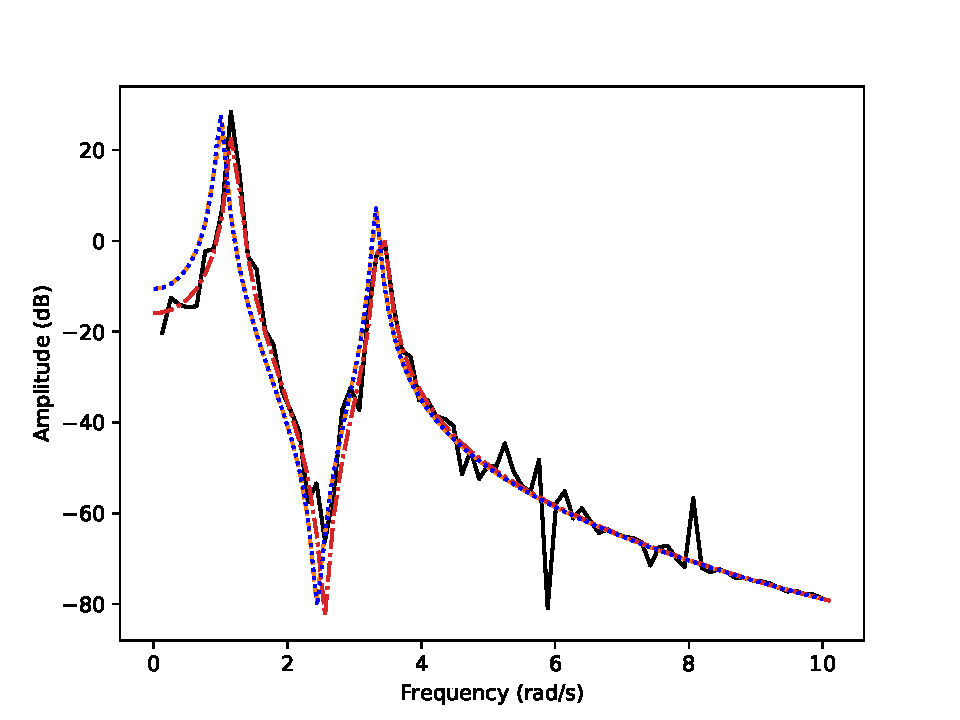
\includegraphics[width=0.8\linewidth]{fnsi/vrms3_H1.tikz}
  \caption{Transfer function $H_1$ for the coupled duffing system.
    \sampleline{}(black): H1 from signal;
    \sampleline{dash pattern=on .7em off .2em on .2em off .2em}\textcolor{red}{(red)}: Linear identified;
    \sampleline{dashed}\textcolor{orange}{(orange)}: Linear identified from FNSI;
    \sampleline{dotted}\textcolor{blue}{(blue)}: Theoretical linear
    % \sampleline{dash pattern=on .7em off .2em on .05em off .2em}
  }
  \label{fig:fnsi_H1}
\end{figure}

\subsection{Estimation error}
\label{sec:fnsi-estimation-error}

It seems that the FNSI method works quite well - both nonlinear and linear
parameters are estimated with high accuracy - and indeed it does work well. But
it is not exact, as will be shown here: the method introduce spurious undesired
terms, and even if they are small in magnitude, they still alters the
identified model.



\subsection{Summary}
\label{sec:summary-fnsi}

The FNSI method is able to identifying multiple nonlinear parameters for system
with many DOFs. It differs from time domain methods, with the ability to
truncate measured signals to the frequency intervals of interest making
computations faster for large systems.

Characterisation of the nonlinearity is important to get a good identification.
If there is limited knowledge about the nonlinearity, cubic splines can be used
instead of polynomials.
In general the following steps can be used to check the validity of the
identification:

\begin{itemize}
\item Check the stabilisation of the first mode.
\item Check the modal parameters compared to linear identification.
\item Check the stability of the nonlinear coefficients versus frequency.
\item Check the magnitude of the imaginary parts of the coefficients.
\end{itemize}


% \begin{table}[h]
% % scale down the table to the textwidth
% \resizebox{\textwidth}{!}{
% %  \begin{tabularx}{\textwidth}{XXX}
%   \begin{tabular}{lll}
%     \hline
%     Property              & TNSI & FNSI \\
%     \hline
%     Domain & Time & Frequency \\
%     MIMO  & Yes & Yes \\
%     Iterative & No & No \\
%     Data exploited & Transient & Steady State \\
%     Data pre-processing & No & DFT \\
%     Frequency-domain data reduction & Not possible & User-selected bands \\
%     Characterization capability & Multiple-term model and {\textit a posteriori}
%                                   discrimination & Identification error criterion\\
%     Stabilization diagram &  Yes & Yes \\
%     Accuracy of the linear parameter estimates   & High, with larger errors on
%                                                    damping ratios & High, with larger
%                                                                     noise variability\\
%     Accuracy of the nonlinear parameter estimates & High, with larger noise variability & High, with larger
%                                                                                           frequency dependence\\
%     Computational burden & Moderate & Low\\
%     \hline
%   \end{tabular}}
%   \caption{Summary of the properties and identification capabilities of the TNSI
%     and FNSI methods, \citet{noel2014a}}
%   \label{tab:tnsi_fnsi_comparison}
% \end{table}


% Question.
% Dear Jean-Philippe,

% I was at your Nolinsys course in september and would like to demonstrate to my
% supervisor, Jon Juel Thomsen, DTU, how you do parameter estimation.
% So following your paper:
%     Method by J.P Noel. Described in article
%     "Frequency-domain subspace identification for nonlinear mechanical systems"
%     http://dx.doi.org/10.1016/j.ymssp.2013.06.034

% I have done steps up till 10, ie. I can estimate/calculate \hat{E, B, C ,D}
% in step 9 but then I don't know what to do about equation (45).
% I have copied t equations, with dimensions, from your article. See the attached pdf.

% So my question is:
% How do I extract H and \mu from eq. 1.2 (45)? I have calculated H^e, but do not
% understand how to proceed.

% Here is a snippet from my code:

% # step 10
% (loop over omegas: I know it is a bit inefficient, this is just to understand your paper.)
% omegas = range(0,100) # just some range of interest
% for idx, omega in enumerate(omegas):
%     He = C.dot(linalg.inv(np.eye(n,dtype=complex)*1j*omega - A).dot(B)) + D
%     # Calculate H, extract mu's and save in matrix
%     H = ?
%     mu[:,idx] = 



% JUST a note:
% I have also looked at your ph.d thesis. There the formulation seems a bit
% different than in the article, ie:
% Q = H [I^(n,n)  -mu_1 * I^(n,n)  ...  -mu_s * I^(n,n)] E = H^e E

% ie. H is just extracted as the first n columns, as you also write.



%%% Local Variables:
%%% mode: latex
%%% TeX-master: "../../report"
%%% End:
